%El autor de este texto es Oscar Abraham Olivetti Alvarez

\chapter{?`Qué es una ley de la naturaleza?}

\noindent En el primer capítulo de este trabajo expusimos brevemente algunas teorías filosóficas de la explicación. Además, hicimos una distinción entre métodos para investigar relaciones causales y los aspectos metafísicos de la causalidad. Ofrecimos razones para tomar a la teoría de Woodward como una buena teoría que describe métodos para investigar relaciones causales. Más aún, la presentamos como una alternativa deseable para trabajar explicación en biología.

Todo lo anterior está relacionado con los aspectos epistémicos de la ciencia. Sin embargo, se puede argumentar que tanto causa como efecto son conceptos intrínsecamente deterministas. Pensemos, por ejemplo en el debate acerca del determinismo. Los deterministas nos dicen que el conjunto de variables en $t_{n}$, en conjunción con las leyes de la naturaleza, causa a $t_{n+1}$. Si causalidad implica determinismo, entonces debemos excluir a las relaciones causales de nuestras explicaciones en biología dada la asimetría entre explicar y predecir. Es en este segundo capítulo nos ocuparemos de dichos aspectos metafísicos de la causalidad y cómo esto está relacionado con las leyes de la naturaleza.

La causalidad y las leyes de la naturaleza son temas estrechamente relacionados en filosofía de la ciencia. Nosotros dijimos en el primer capítulo que las leyes no son necesarias para la explicación. Sin embargo, aquellas que toman una postura realista de las leyes podría argumentar que las leyes describen conexiones necesarias y que con la teoría de Woodward simplemente estamos dejando de lado este aspecto.

Hay al menos tres grandes posturas en el debate acerca de las leyes de la naturaleza \cite{Borge2019}. Por un lado, están los humeanos sobre las leyes: quienes afirman que las leyes no describen conexiones necesarias en el mundo. Podemos pensar a los humeanos como la postura anti-realista de las leyes. Por otro lado los necesitaristas afirman que las leyes de la naturaleza son descripciones de cómo el mundo de hecho se comporta, por lo que la modalidad de las leyes refleja una propiedad del mundo: hay conexiones necesarias en el mundo. Por último están los disposicionalistas. Los disposicionalistas ponen énfasis en las propiedades que tienen los objetos, para ellos, lo que hacen las leyes de la naturaleza es relacionar propiedades. Los disposicionalistas afirman que las propiedades no son inertes, sino modalmente activas.

Dependiendo de lo que tomemos como primitivo, habrá repercusiones en otros debates sobre metafísica de la ciencia. Si tomamos \emph{necesidad} como primitivo y las leyes se encargan de describir relaciones necesarias entre objetos, entonces podemos decir que las leyes describen relaciones causales. Estas relaciones serán a su vez necesarias tal como son descritas por las leyes naturales. Más aún, un antihumeano sobre las leyes puede argumentar a favor del determinismo causal. Debido a que ya ofrecimos razones para tomar al modelo de Woodward como una buena teoría de la explicación, ahora queremos posicionarnos sobre el aspecto metafísico de las leyes de la naturaleza que defenderemos a la par del modelo de Woodward.

Esto es importante porque regularmente se toma como evidencia a favor de las tesis anti-humeanas el hecho de que las leyes son enunciados que describen las conexiones necesarias del mundo. En esta postura las leyes no son sólo descripciones, sino que gobiernan cómo el mundo se comporta\cite{Bhogal2020}. Otra postura defenderá necesidad al nivel de las propiedades, estos son los disposicionalistas. La alternativa humeana, contraria a estas dos posturas, es el famoso mosaico del que habla Lewis\footnote{El mosaico humeano se refiere a la configuración espacio-temporal de eventos concretos: un evento sucede, y después otro evento sucede.}. Los humeanos, como Lewis, argumentan que hay una relación de superviniencia entre el mosaico humeano y las leyes de la naturaleza.

%Una necesitarista sobre las leyes puede argumentar que, si bien la teoría de Woodward ofrece un método para rastrear casuas, aún es compatible con el hecho de que haya necesidad en el mundo. Las leyes decriben cómo se comporta el mundo y es un defecto de la teoría sólo centrarse en relaciones invariantes bajo intervenciones. En este capítulo queremos argumentar que la necesidad de las leyes se deriva de nuestras teorías y nuestros modelos.

Podemos llevar a cabo muchas de nuestras tareas epistémicas sin tener que recurrir a leyes. Es decir que en lo siguiente nos dedicaremos a reflexionar sobre la parte metafísica de las leyes, no sobre su carácter en tanto dispositivos útiles para explicar. Hay que tener en cuenta que regularmente se dice que las leyes capturan conexiones causales entre fenómenos. Por lo que lo que digamos aquí sobre las leyes, tiene consecuencias en nuestras teorías de la causalidad.

Nuestro argumento es modesto. Procedemos de la siguiente manera: primero exponemos que el nacimiento del término ``ley de la naturaleza'' indica que los necesitaristas deben secularizar el término. Luego proponemos los criterios de Nagel como una buena manera de secularizar el término. Después exponemos dos casos que intuitivamente diríamos que son leyes de la naturaleza. Argumentamos que la necesidad que expresan estas leyes no es algo que esté en el mundo, sino que depende de los modelos en los que se inscriben. El argumento concluye en que si bien pueden ser necesarias dentro de un modelo, las leyes no rastrean relaciones necesarias en el mundo natural. Lo que llamamos ``leyes de la naturaleza'' son aplicaciones de un formalismo particular y es de este formalismo del que surge una necesidad aparente.

\section{El nacimiento del término}

\noindent El concepto de ``ley de la naturaleza'' ha estado presente en los debates filosóficos acerca de la metafísica de la ciencia, la epistemología de la ciencia y los objetivos de la ciencia. Nos interesa, por un lado, una caracterización de qué \textbf{son} las leyes; por otro lado cómo nos sirven para explicar y cómo obtenemos evidencia de ellas (tanto su papel en la explicación como los métodos de obtención de evidencia son debates marcadamente epistémicos); aunado a esto, también se suele afirmar que el objetivo de la ciencia es buscar las leyes de la naturaleza.

%Con respecto al primer punto, Nagel nos ofrece una caracterización. El segundo punto está estrechamente relacionado con el modelo de explicación de Hempel, que padece de los problemas que revisamos en el primer capítulo. El último factor tiene un peso intuitivo, pero Giere \citeyear[p. 69]{Giere2006} menciona que las leyes de la naturaleza no son ``parte literal del contenido de ninguna ciencia. [Las leyes de la naturaleza] son una noción que pertenece a un meta-nivel de interpretación acerca de lo que hacen los científicos''\footnote{[...] a law of nature is not part of the literal content of any science. It is a notion that belongs to a meta-level interpretation of what scientists do [...].}. Por lo que podemos concentrarnos en el estatus metafísico de las leyes de la naturaleza. El argumento que expondremos es marcadamente sobre la ontología de las leyes, es decir, de lo que las leyes \textit{son}.

Pasando al uso del término, el término ley de la naturaleza comenzó a ser utilizado a principios del siglo XVII. En su origen el término estuvo ligado a la teología y a la jurisprudencia \cite{Giere2006, Giere1999}. Evidencia de esta relación con la jurisprudencia la encontramos en la entrada de leyes de la naturaleza en la enciclopedia de d'Alambert y Diderot \cite{lawna}. Más aún, en la entrada se menciona que primero se llegó a pensar que las leyes naturales son aquellas impuestas por Dios para la buena conducta de los seres humanos. Si se actúa de acuerdo a los deseos de Dios, entonces las acciones son buenas. Además, Dios dota con conocimiento a los seres humanos. Los seres humanos al estar dotados de conocimiento, somos capaces de conocer esas leyes al examinar la naturaleza. Esto nos da evidencia del origen del término y su uso: en el siglo XVII las leyes de la naturaleza son las leyes de Dios, y en esto recae la afirmación de que sean necesarias.

Si el término de ley de la naturaleza está ligado a la teología, los anti-humeanos tendrían algo que decir al respecto de esto: dudamos que alguna anti-humeana actual quiera aceptar que las leyes de la naturaleza son las leyes de Dios. Hay al menos dos soluciones que se nos ocurren. La primera es aceptar que ley de la naturaleza es de hecho un término teológico, o bien decir que, si bien el origen de las leyes es iluminador, no captura el significado de ``ley de la naturaleza'' que nos interesa ahora. Después de todo, los términos cambian y no se está utilizando el término ``leyes de la naturaleza'' en el sentido que lo entendemos actualmente.

En particular, nosotros estaríamos de acuerdo con esta última línea de argumentación. El hecho de que el origen del término esté cargado de teología (y, por tanto, desearíamos excluirlo de la investigación científica actual), no implica que sea así necesariamente. Es decir, se puede secularizar el término. Una manera descargar a la teología del término es adoptando como alternativa las características que da Nagel: i) debe ser un universal irrestricto, es decir, que funciona en todo momento para una cantidad potencialmente infinita de objetos; ii) en su formulación sólo debe haber vocabulario puramente cualitativo, esto con el fin de evitar que se haga referencia a objetos en un espacio y tiempo determinados y iii) debe haber algún tipo de relación tal que el antecedente haga necesario el consecuente. Si esto es correcto, entonces lo que resta es ver si existen enunciados que funcionen a la manera descrita por Nagel. Dedicaremos la siguiente sección a ello.

\section{Modelos y necesidad}

\noindent Comencemos tomando un ejemplo de la biología. En Losos \emph{et al.}\citeyear{Losos2004} se quiere investigar qué sucede con el proceso evolutivo de la especie \textit{Anolis sagrei} cuando se introduce un depredador, en específico el \textit{Leiocephalus carinatus}. \textit{A. sagrei}  es un tipo de lagartija, mientras que \textit{L. carinatus} es un tipo de lagarto, ambos habitantes de las islas de Cuba.

Sucede que al introducir a este depredador, que habita principalmente en el suelo, el \textit{A. sagrei} tiende a habitar lugares más altos y sus extremidades se desarrollan de manera tal que le permitan escalar. Esto responde a la pregunta ¿por qué \textit{A. sagrei}, que suele ser una lagartija que habita en los suelos, comenzó a desarrollar extremidades que le permitan escalar? Cuya respuesta es ``porque se introdujo un depredador que principalmente habita en el suelo''.

La anterior es una explicación según el modelo de Woodward: introducir a un depredador, genera un cambio en la presa. Además, la práctica científica acepta esta explicación como tal. A pesar de ello, no hay leyes en su formulación y no parece plausible generar una ley a partir de este caso particular. Sin embargo, aún queda el hecho de que podrían ser suficientes para la explicación y, por tanto, favorecer a la postura anti-humeana. El argumento de esta sección descansa en que las leyes no capturan conexiones necesarias como lo requiere el anti-humeano.

Para hacer una distinción entre leyes y generalizaciones accidentales, supongamos por ejemplo que tengo una leve obsesión con las monedas de \$1 y que en mi bolsillo siempre llevo al menos 5 monedas de \$1. En este caso, el enunciado ``todas las monedas del bolsillo de Abraham son de \$1'' sería verdadero, pero no lo consideramos una ley. Un caso que parece tener las características de ser una ley es el siguiente: cuando afirmamos que todos los trozos de cobre se dilatan al calentarse.  Con esta afirmación, queremos decir algo más que ``no hay un pedazo de cobre que no se dilate al calentarse''. Se quiere capturar cierto tipo de conexión entre el que algo sea de cobre y que se dilate al calentarse. Esta conexión, al menos en la literatura clásica, es necesidad: el hecho de que el material sea cobre, hace necesario que se dilate al calentarse. Este enunciado es distinto a mi ejemplo de las monedas. Los anti-humeanos dirán que el enunciado sobre el cobre es una ley de la naturaleza, mientras que el enunciado sobre las monedas no lo es.

La postura de Nagel sobre las leyes tiene como componente una relación en la que el antecedente hace necesario al consecuente. Es por ello que Nagel dice que lo que hace falta en casos como el del cobre es hacer una demostración de la necesidad de dicha conexión. No es claro que en los casos de las monedas y el de \emph{A. sagrei} tengamos una ley. El caso del cobre parece ser un mejor candidato de ley de al naturaleza. Sin embargo, esta relación de necesidad nos lleva a un problema. Según Nagel, las leyes son necesarias, pero además tenemos la intuición de que las disciplinas científicas trabajan empíricamente. Nagel mismo menciona que no sería deseable que la ciencia proceda en términos de prueba necesaria a la manera en como lo hace la geometría \cite[cfr., p. 53]{Nagel2006} porque se perdería el componente empírico de la ciencia. Esto significa, para Nagel, que: o bien las leyes son necesarias y perdemos el componente empírico de la ciencia, o bien las leyes no son más que contingentes y mantenemos el compromiso empírico de la ciencia.

Suponiendo que el enfoque de Nagel es una buena manera de secularizar el término ``ley de la naturaleza'', queremos decir que el dilema que Nagel presenta es un falso dilema. Hay casos históricos que intuitivamente diríamos que son leyes de la naturaleza, que proceden a la manera geométrica y que además no pierden el componente empírico. Nos centraremos en mostrar dos casos que harán que este dilema desaparezca. Esto a su vez presenta un caso contra quien defienda una tesis anti-humeana de las leyes, ya que diremos que la necesidad involucrada es parte de la prueba y no algo que esté el la naturaleza.

No es grave el hecho de que se trabaje con generalizaciones contingentes. En lo expuesto en el capítulo anterior argumentamos en favor de que un buen modelo de explicación es el que nos presenta Woodward. Este modelo no necesita leyes a la manera tradicional, es decir, enunciados universales verdaderos y con contenido empírico. Sin embargo, aún resta atacar la fuerte intuición de que las leyes son necesarias. Creemos que esta aparente necesidad no es algo propio de los objetos que están relacionados en las leyes, sino del método con el cual las construimos. Creemos que la aparente necesidad se debe justo a la construcción geométrica de algunas de las leyes: en especial las de Arquímedes y Galileo. Pero esta necesidad en las leyes no es el tipo de necesidad que necesita la anti-humeana para sostener su postura. Recordemos que la anti-humeana pone el carácter modal de las leyes en las relaciones entre objetos.

\section{La necesidad en las leyes}

\noindent Empecemos por explorar la afirmación de Nagel de que el proceder científico perdería su parte empírica si procediera como lo hace la geometría. Cuando decimos que algo procede a la manera geométrica, por lo general nos referimos al método que utiliza Euclides en los \emph{Elementos} \cite{Euclid2008}. Cuando decimos que algo procede a la manera geométrica, estamos sosteniendo la tesis de que cualquier consecuencia del sistema es derivable de las definiciones y las nociones comunes a las que se refiere Euclides. Todos los libros que conforman los \emph{Elementos} tienen la misma estructura. En particular, nos interesa  el libro 5 que es donde Euclides expone la teoría de proporciones.

Detengámonos por un momento y pensemos a la teoría de proporciones como un modelo formal. Es decir que cuando interpretamos a la teoría\footnote{El proceso en el que sustituimos las variables de las que habla Eucldies por constantes. En el caso de Galileo las constantes son distancia y tiempo, en el caso de Arquímedes las constantes son pesos y distancias. Este proceso es una interpretación de la teoría}, manetenemos las relaciones sintácticas entre los enunciados. Euclides comienza el libro 5 dándonos un conjunto de definiciones y es a partir de estas definiciones que extrae una serie de teoremas.

La teoría de proporciones fue utilizada por Arquímedes y tiempo después por Galileo para derivar teoremas para su teoría ``sustituyendo'' los objetos de los cuales habla la teoría de proporciones con otro tipo de objetos. Nuestra apuesta es que la teoría de proporciones es un modelo formal al que se puede interpretar con diferentes objetos y qeu al ser expresadas en la teoría formal, la necesidad surge de su calidad de teoremas\footnote{Recordemos que una derivación no hace necesario al enunciado. Supongamos por ejemplo que hoy traigo puesto un sombrero. Esto implica que hay algo que trae un sombrero. Sin embargo no implica que necesariamente algo trae un sombrero. Lo que es necesario es el esquema argumental, es decir si asumimos la verdad del antecedente, entonces se sigue el consecuente. Esto es lo que queremos decir en analogía con el caso de la teoría de proporciones euclideana.}.

Tarski definió en términos formales qué es un modelo y cómo esto nos ayuda a aclarar el concepto de consecuencia lógica \cite{Tarski1956}. Tarski se preocupa por al menos tratar de recuperar dos nociones importantes del concepto de consecuencia lógica: necesidad y forma \cite{Torrente2000}. Tarski busca que todos los esquemas con la misma forma lleven a las mismas consecuencias. Pero además, hay un sentido importante en que esto es así necesariamente: no es posible que las premisas sean verdaderas, tenga una forma válida y que la conclusión sea falsa. Por lo que hay un componente modal en las derivaciones dentro de modelos formales.

Mencionamos esto de Tarski porque hay una analogía con la teoría de proporciones. Sabemos que de las definiciones que Euclides postula, se siguen los teoremas que deriva en su libro 5. Los modelos de esta teoría son cualquier teoría que pueda ser expresada en términos de la teoría de proporciones. Si esto es verdad, entonces no es un misterio de dónde proviene la intuición de que las leyes son necesarias, son necesarias porque dependen de un aparato formal y las derivaciones son teoremas. La parte empírica depende sólo de con qué constantes sustituyamos las variables. Es decir que la naturaleza \emph{necesaria} proviene de ser derivaciones, mientras que la parte empírica proviene de hacer las sustituciones con objetos.

A continuación discutimos dos ejemplos que muestran que la necesidad proviene directamente de la teoría de proporciones. Galileo en la tercera jornada prueba 6 teoremas acerca del movimiento uniforme y demuestra que si un móvil con movimiento uniforme recorre dos espacios, esos espacios serán entre sí como las velocidades \cite[p. 215]{galtre}. Todo esto expresado en términos de la teoría de proporciones.

Galileo comienza la exposición de la tercera jornada de los \emph{Diálogos Acerca de Dos Nuevas Ciencias} dando una definición y cuatro axiomas del movimiento uniforme. Galileo define al \textit{movimiento uniforme} como aquel movimiento que en los mismos periodos de tiempo recorre el mismo espacio. Es decir que si tenemos una línea dividida en segmentos iguales, durante cada uno de estos segmentos por los que pasa un móvil, el tiempo transcurrido es igual para todos los segmentos.

A parir de esta definición, Galileo nos presenta una serie de \textit{axiomas} que son consecuencias de la anterior definición. En estos axiomas, se dan una relación de desigualdad entre las magnitudes involucradas en el movimiento uniforme. El primer axioma señala que si dos objetos, digamos $A$ y $B$ tienen el mismo movimiento uniforme, entonces si $A$ se desplaza durante más tiempo, la distancia recorrida también será mayor a la de $B$. Nos dice también que para el mismo movimiento uniforme, si el tiempo transcurrido es mayor, también lo será la distancia. Después de estos axiomas, Galileo se dispone a demostrar una serie de teoremas.

Supongamos que los axiomas y las definiciones ofrecidas por Galileo son necesarios. Con esto queremos decir que al menos se pueden expresar en cualquier mundo posible para evitar el compromiso de si describen o no correctamente el comportamiento dle mundo. Si los axiomas y definiciones son necesarios, se sigue necesariamente que las distancias son proporcionales a los tiempos, como muestra el siguiente ejemplo.

En el primer teorema Galileo demuestra que si un móvil con movimiento uniforme recorre dos distancias, esas distancias serán entre sí como los tiempos \cite[p. 215]{galtre}. Galileo nos pide que consideremos que un móvil recorre con velocidad constante dos distancias. Se nos pide que consideremos una distancia $AB$ y una distancia $BC$. Consideremos además los tiempos correspondientes para atravesar ambas distancias $DE$ y $EF$ respectivamente. Extendamos los segmentos $BA$ y $BC$, de manera que $AG$ y $CH$ sean múltiplos de $AB$ y $BC$ respectivamente. Extendamos a su vez los tiempos $DE$ y $EF$ hacia $FK$ y $DI$, donde $FK$ y $DI$ son múltiplos iguales de $AG$ y $CH$ respectivamente.

$DE$ es el tiempo que tarda un móvil en recorrer la distancia $AB$ y debido a que el movimiento es uniforme, entonces cualquier equimúltiplo arbitrario de $AB$, en este caso $AG$, $DI$ será el tiempo total que tarda en recorrer $AG$. Entonces si $AG > BH$, $DI > FK$; si $AG = BH$, $DI = FK$; si $AG < BH$, $DI < FK$. Por tanto, según la definición cinco\footnote{``Decimos que las magnitudes tienen la misma razón, la primera a la segunda y  la tercera a la cuarta, cuando múltiplos iguales de la primera y la tercera, en conjunto: o bien exceden, o bien son iguales, o bien son menores que múltiplos iguales de segunda y la cuarta''} del libro V de Euclides \cite{Euclides1956} $AB:BC$ tiene la misma razón que $DE:EF$ y son proporcionales dada la definición seis del mismo libro, que es lo que se quería probar.

Esto quiere decir que si son necesarios los axiomas y de los axciomas se sigue que los tiempos son proporcionales a las distancias, entonces este último resultado es a su vez, necesario. Pensemos en otro ejemplo.

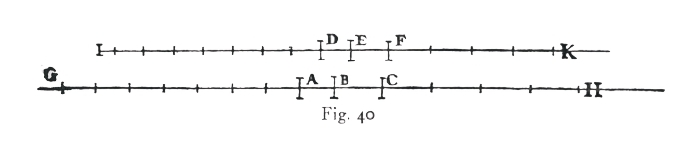
\includegraphics[width=\textwidth]{fig40.jpg}

El segundo ejemplo es lo que hace Arquímedes en \emph{Sobre el equilibrio de los cuerpos planos} \cite{Archimedes1897}. Arquímedes utiliza la teoría de proporciones para probar una serie de teoremas que relacionan a los pesos y a las distancias. El libro comienza con una serie de postulados. Entre los postulados de Arquímedes encontramos que: pesos iguales a distancias iguales estarán en equilibrio. Si dos objetos están en equilibrio y se agrega más peso a uno de los lados, entonces se inclinará hacia el cual se le agregó el peso. Si dos pesos están en equilibrio y quitamos peso de uno de los lados, entonces se inclinará hacia el lado donde el peso se mantuvo. El primer teorema nos dice que si hay dos pesos a distancias iguales, entonces los pesos son iguales. Si hay dos pesos diferentes a distancias iguales, entonces se inclinará hacia el de mayor peso. Prueba: quítese del peso mayor la diferencia entre ambos, entonces se equilibrarán y, si volvemos a poner el peso que hemos quitado, se balanceara hacia el que se agregó el peso.

Si estamos ante el mismo fenómenos y una vez aceptamos las definiciones y axiomas tanto de Galileo como de Arquímedes, entonces aceptamos los resultados. En analogía con lo expuesto por Tarski hay un carácter de necesidad involucrado al ser derivaciones que dependen de la teoría que Euclides desarrolla en el libro V de los elementos. Si estamos jugando en el mismo terreno y aceptamos\footnote{Aquí hay una relación entre aceptar como verdaderos los axiomas. Esto se debe a que es sólo cuando aceptamos que son verdaderos que podemos hacer la derivación del consecuente. No nos meteremos en el tema de los axiomas y sus condiciones de evaluación. Lo que queremos poner de relieve es que es cuando asumimos la verdad de los axiomas que podemos derivar a los teoremas que prueban tanto Galileo como Arquímedes.} los axiomas y definiciones que cada uno de ellos propone, tendríamos que decir o bien que alguna de las premisas es falsa, o bien que la derivación es incorrecta. Pero la prueba de Galileo no tiene pasos incorrectos. La otra opción nos lleva directo a un problema en filosofía de las matemáticas acerca de lo que constituye un buen axioma, que es un problema que requiere un trato más extenso del que podemos ofrecer aquí. Lo único que queremos poner de relieve es que la necesidad de las leyes (al menos los ejemplos mostrados aquí) proviene de que son derivaciones de una teoría formal, a la que le hicimos un modelo, por tanto, la necesidad no es algo intrínseco al mundo natural.

%En el siguiente apartado me dedico a explorar el segundo cuerno del dilema que nos presentó Nagel e intentaré justificar la conclusión de que no es necesaria una teoría general que capture todas las características de lo que es una ``ley de la naturaleza'' para rescatar los criterios epistémicos que distinguen a la ciencia.

Nagel afirma que requerir que las ciencias procedieran a la manera de pruebas geométricas, implicaba que se perdiera el componente empírico de la ciencia (que es una fuerte intuición acerca del proceder de la ciencia). Argumentamos que los ejemplos de Galileo y de Arquímedes muestran que esta necesidad no es propia del mundo natural, sino de una teoría formal. Siendo los casos de Galileo y Arquímedes instancias que toman la teoría formal y sustituyen variables por constantes para hacer un modelo. Es en la parte interpretativa de la teoría que mantenemos su carácter empírico y es en la parte de la derivación que mantenemos su carácter de necesidad. Esto quiere decir que las leyes de la naturaleza no son necesarias porque haya algo en la naturaleza que implique conexiones necesarias, por lo que la tesis anti-humeana carece de evidencia para afirmar que la causalidad implica una conexión necesaria.

Esto nos lleva directamente a afirmar el otro disyunto del dilema de Nagel, esto es, el humeanismo acerca de las leyes, y al negar que haya conexión necesaria, entonces vamos al indeterminismo en causalidad. Este punto de acción no es tan grave porque, como mencionamos en el primer capítulo, no necesitamos tener generalizaciones universales para poder explicar. Según la teoría de Woodward es suficiente con tener generalizaciones que sean invariantes.

\section{El estatus de las leyes de la naturaleza}

\noindent Afirmar que las ``leyes de la naturaleza'' no son necesarias no es tan controversial como lo parece a primera vista. Esto no es terreno completamente inexplorado. Por ejemplo, Cartwright \citeyear{Cartwright1983} argumenta que las leyes de la física son literalmente falsas y que sólo se cumplen en casos muy concretos en los que se dan las condiciones adecuadas para que la ley ocurra tal como se describe. Fuera de estos casos, difícilmente veremos a la naturaleza comportarse como describen las leyes de la naturaleza. Esta autora asegura que es esto lo que le da la fuerza explicativa a la teoría. Cartwright asegura que la ley de la gravitación universal es falsa ya que siempre hay otras fuerzas actuando y que es sólo cuando se agrega la cláusula \textit{ceteris paribus} que dicha ley es verdadera. Pero al hacer que la ley sea verdadera perdemos poder explicativo.

Elgin presenta un punto semejante al de Cartwright. Elgin \citeyear{Elgin2004} señala que estamos en un dilema cuando hablamos de verdad en ciencia: o bien hacemos más laxos nuestros compromisos con la verdad, o bien aceptamos que la ciencia es deshonesta y epistémicamente deficiente. Elgin nos presenta varios casos en los que los científicos aceptan ``falsedades'' porque tienen virtudes cognitivas, en contraste con tener una descripción literalmente verdadera. En algunas ocasiones nos interesa interpretar datos o dar cuenta de fenómenos aún cuando no sea una descripción literalmente verdadera. Una manera de clarificar esto es el caso que nos presenta la autora sobre la ley de Snell. La ley de Snell nos dice que el ángulo de refracción de la luz, cuando un rayo de luz pasa de un medio a otro, es el ángulo de incidencia multiplicado por el índice de refracción del primer medio y esto es igual al ángulo de refracción multiplicado por el índice de refracción del segundo medio. Elgin señala que esta ley es útil, pero es falsa porque no se cumple para todos los casos, sino sólo para aquellos casos en que los medios de propagación son isotrópicos.

En este caso Elgin nos dice que si bien la ley es falsa, la utilizamos porque tiene un valor epistémico que perderíamos si buscáramos que la ley fuera verdadera (por ejemplo, acotando el dominio de discurso sólo al caso de los medios isotrópicos), estas virtudes dependen de su falsedad y de qué tanto se desvía de una descripción literalmente verdadera de la realidad. Al darnos cuenta de dicha desviación, aprendemos algo sobre los medios por los que atraviesa la luz.

Ambas posturas tienen un fuerte compromiso con el hecho de que las leyes de la naturaleza son literalmente falsas. Creo que podemos hacer sentido de esta falsedad con el marco desarrollado en este capítulo. En primer lugar, la conclusión es que las leyes son necesarias en tanto que son derivaciones. Hay otro tipo de generalizaciones que no son necesarias, como en el ejemplo de \emph{Anolis sagrei}. Debido a que las leyes no son necesarias en virtud de reflejar conexiones necesarias del mundo natural, entonces es claro que las leyes pueden fallar, por ejemplo, cuando desechamos alguno de los axiomas o definiciones. Esto les concede el punto a Cartwright y Elgin.

Sin embargo, detengámonos un momento en las afirmaciones de Cartwright y Elgin. Ambas autoras hacen de la verdad un objetivo secundario de la ciencia y que parecen hacer del ``poder explicativo'' el valor epistémico fundamental\footnote{Haría falta revisar exactamente a qué se refieren con poder explicativo. Si se refieren a que estos enunciados ayudan a explicar cómo suceden los fenómenos, entonces tendrían que describir correctamente el comportamiento de los fenómenos. Pero esto sólo lo podemos asegurar si la descripción es verdadera. Volviendo de nuevo al problema del que trataban de deshacerse.}. Si bien concedemos a Cartwright y Elgin que las leyes sólo son literalmente verdaderas cuando se cumplen un montón de cláusulas \emph{ceteris paribus}, nos parece que modificar nuestros compromisos con la verdad con otro tipo de valores epistémicos es un paso apresurado. Por lo que aún hay algo que explicar acerca de cómo la verdad juega un papel en la investigación científica.

\section{El papel de la verdad en la investigación}

\noindent En un artículo reciente \cite{Pritchard2019}, Pritchard argumenta que el paso de tener a la verdad como un valor epistémico secundario no resuelve los problemas que pretende. Pritchard explora la tesis de que la verdad es el valor epistémico por excelencia y desarrolla un argumento que trata de resolver los problemas que parece tener la afirmación ``la verdad es el único valor epistémico fundamental''.

Una razón para decir que la verdad no es fundamental, o bien no es el único valor importante, parece ser el hecho de que cualquiera que valore la verdad, valorará todas las verdades por igual. Por poner un ejemplo burdo, seguro hay una respuesta correcta a la pregunta ¿cuántos ladrillos hay en las paredes de mi casa?, pero sería ocioso perseguir esta respuesta. Pero si la respuesta es necesaria, digamos porque necesito derribar mi pared y construirla de nuevo, entonces la respuesta adquiere un valor.

Hay una respuesta verdadera a la pregunta y es valioso perseguirla sólo cuando es necesaria. Es en este punto en donde recae el valor de la verdad. En el caso de los modelos, nos son útiles cuando se puede aislar un factor que determina el comportamiento del fenómeno que estamos estudiando. El modelo de Woodward es capaz de hacer esto.

Es capaz de hacerlo en tanto que nos ayuda a aislar componentes causales de los fenómenos bajo escrutinio al modificar ciertas variables y analizar el comportamiento de las otras variables. Una objeción que se nos ocurre es que en los ejemplos de Galileo y de Arquímedes, no es claro cómo vamos a aislar un componente. Sin embargo, hay muchas maneras de pensar estos ejemplos en términos del modelo de Woodward.

Piénsese por ejemplo el caso en el que variamos el hecho de que sea un movimiento uniforme. Cuando el movimiento no es uniforme, entonces no se sigue que las distancias son proporcionales a los tiempos. Más aún, el modelo de Woodward se puede extender lo suficiente como para preguntarnos qué pasaría si utilizáramos una teoría diferente a la teoría de proporciones de Euclides \cite{Woodward2018}. Al hacer esto aislamos un factor, no necesariamente causal, y podemos describir el comportamiento de fenómenos naturales.

Pritchard nos dice que la proposición no es el único objeto que carga valor epistémico al ser verdadero. Digamos que tenenemos dos respuestas correctas a dos preguntas diferentes, llamémoslas P y Q. Una de las preguntas es trivial y la otra es ``de más peso''. Si lo único que estuviera en juego fuesen P y Q, entonces tendríamos el problema mencionado antes. Pero no es claro por qué cualquiera que acepte que la verdad es un valor fundamental debería aceptar esto. Podría argumentarse que no importa sólo que una proposición sea verdadera, sino que las proposiciones vinculadas a ella también lo sean. Si el resultado permite obtener más verdades, entonces será un resultado más valioso. Pritchard apela a la teoría de virtudes epistémicas\footnote{Las virtudes epistémicas son capacidades de los agentes que se desarrollan con el hábito. Entre algunas podemos nombrar: que el agente sea observador, que preste atención a la evidencia, que tenga buena memoria, etc. Esto hace que las otras virtudes que probablemente juegan un papel como valores epistémicos, estén dependan del agente y no de valores como los que describen las tesis de Cartwright y Elgin.} y hace que este último punto dependa del agente. Podemos asumir que el agente es virtuoso y se preocupa por la verdad. Los agentes además tienen intenciones, por lo que de acuerdo a qué preguntas necesite responder, podrá elegir qué necesita investigar. Este desarrollo que hace Pritchard podría ayudar a explicar cómo es que la verdad juega un papel en la investigación científica.

En este capítulo hemos argumentado que la aparente necesidad de \textbf{algunas} leyes deriva del hecho de que son modelos de una teoría formal: la teoría de proporciones. Esto es sólo un poco de evidencia a favor de la tesis humeana sobre las leyes de la naturaleza: la necesidad depende de un marco formal, no de conexiones en el mundo. Si todo esto es correcto, entonces la necesitarista (aquella que afirma que hay necesidad en algunas conexiones naturales) o alguna otra defensora de alguna teoría no-humeana de las leyes, como la disposicionalista, está en serios problemas para dar cuenta de las conexiones causales.

Aunado a esto, nos parece que el modelo de Woodward es una buena alternativa para una teoría general de la explicación y una teoría general de la causalidad. Lo que resta en este trabajo es una aplicación concreta de lo dicho hasta ahora. En el siguiente capítulo nos proponemos analizar el debate de la naturaleza del \emph{fitness}. Creemos que lo dicho hasta ahora ofrecer claridad en torno a este debate.

%El autor de este texto es Oscar Abraham Olivetti Alvarez
